% Gabarit pandoc des corrigés publiés (brut et guidé). Contenu sans marque ni nom de site.
% Compilation : lualatex (latexmk -lualatex).
% Le Markdown reste la source unique : ne pas éditer ce fichier .tex à la main.
\documentclass[11pt,a4paper]{article}

% --- Moteur, polices (Latin Modern) et langue ---------------------------------
\usepackage{iftex}
\ifLuaTeX\else\errmessage{Ce document se compile avec lualatex}\fi
\usepackage{amsmath,amssymb,mathtools}
\usepackage{fontspec}
% mathrm=sym : \mathrm prend ses glyphes dans la police mathématique (ℓ, μ, Ω), comme KaTeX.
\usepackage[math-style=TeX,bold-style=TeX,mathrm=sym]{unicode-math}
% Repli pour les glyphes absents de Latin Modern (indices et exposants Unicode,
% flèches, filets des schémas en texte, symboles) : DejaVu, puis Latin Modern Math
% (ℓ, lettres mathématiques Unicode des légendes).
\directlua{
  luaotfload.add_fallback("repliTexte", {"DejaVuSerif:mode=harf;", "DejaVuSans:mode=harf;", "file:latinmodern-math.otf:mode=harf;"})
  luaotfload.add_fallback("repliMono", {"DejaVuSansMono:mode=harf;", "DejaVuSans:mode=harf;", "file:latinmodern-math.otf:mode=harf;"})
}
\setmainfont{Latin Modern Roman}[RawFeature={fallback=repliTexte}]
\setsansfont{Latin Modern Sans}[RawFeature={fallback=repliTexte}]
\setmonofont{Latin Modern Mono}[RawFeature={fallback=repliMono}]
\setmathfont{Latin Modern Math}
\usepackage[french]{babel}
\frenchsetup{SmallCapsFigTabCaptions=false}

% --- Mise en page --------------------------------------------------------------
\usepackage[a4paper,margin=2.2cm,headheight=14pt,footskip=1.2cm]{geometry}
\usepackage{microtype}
\setlength{\emergencystretch}{4em}
\tolerance=1500
\setlength{\parindent}{0pt}
\setlength{\parskip}{0.55\baselineskip plus 2pt minus 1pt}
\usepackage{xcolor}
% Gris nommés : babel-french rend « ! » actif dans le document.
\definecolor{gris2}{gray}{0.98}
\definecolor{gris3}{gray}{0.97}
\definecolor{gris5}{gray}{0.95}
\definecolor{gris35}{gray}{0.65}
\definecolor{gris40}{gray}{0.60}
\definecolor{gris45}{gray}{0.55}
\definecolor{gris50}{gray}{0.50}
\definecolor{gris55}{gray}{0.45}
\definecolor{gris60}{gray}{0.40}
\definecolor{gris65}{gray}{0.35}
\definecolor{gris70}{gray}{0.30}
\definecolor{gris80}{gray}{0.20}
\definecolor{gris85}{gray}{0.15}
\usepackage{graphicx}
\usepackage{float}
\usepackage{caption}
\captionsetup{font=small,labelformat=empty,justification=centering}
\usepackage{booktabs,longtable,array,multirow,calc}
\usepackage{siunitx}
\sisetup{locale=FR}
\usepackage[version=4]{mhchem}
\usepackage{listings}
\usepackage{fancyhdr}
\usepackage{lastpage}
\usepackage[most]{tcolorbox}
\usepackage{enumitem}
\setlist{nosep,leftmargin=*,topsep=2pt}
\usepackage[hidelinks,unicode]{hyperref}
\usepackage{bookmark}
\hypersetup{pdftitle={Banque PT — Mathématiques A 2026},pdfauthor={Rédigé par IA},pdfcreator={LaTeX},pdfsubject={Corrigé brut}}
\usepackage{xurl}

% --- Pandoc : listes, tableaux, figures ----------------------------------------
\providecommand{\passthrough}[1]{#1}
\providecommand{\tightlist}{\setlength{\itemsep}{0pt}\setlength{\parskip}{0pt}}

\makeatletter
\def\maxwidth{\ifdim\Gin@nat@width>\linewidth\linewidth\else\Gin@nat@width\fi}
\def\maxheight{\ifdim\Gin@nat@height>0.55\textheight 0.55\textheight\else\Gin@nat@height\fi}
\makeatother
\setkeys{Gin}{width=\maxwidth,height=\maxheight,keepaspectratio}
\setcounter{secnumdepth}{-\maxdimen}
\providecommand{\pandocbounded}[1]{#1}
\usepackage{longtable,booktabs,array}

% --- Code (listings) -----------------------------------------------------------
\lstset{
  basicstyle=\ttfamily\small,
  columns=fullflexible,
  keepspaces=true,
  breaklines=true,
  breakatwhitespace=false,
  postbreak=\mbox{\textcolor{gris50}{$\hookrightarrow$}\space},
  frame=single,
  rulecolor=\color{gris35},
  framesep=4pt,
  xleftmargin=5pt,xrightmargin=5pt,
  backgroundcolor=\color{gris3},
  keywordstyle=\bfseries,
  commentstyle=\color{gris65},
  stringstyle=\color{gris80},
  showstringspaces=false,
  tabsize=4,
  extendedchars=true,
  aboveskip=6pt,belowskip=6pt,
}

% --- Macros des corrigés (KaTeX ↔ LaTeX) ---------------------------------------
% Les corrigés sont écrits pour KaTeX : on définit ici ce que KaTeX connaît et
% que LaTeX n'a pas, sans jamais retoucher le Markdown.
\providecommand{\R}{\mathbb{R}}
\providecommand{\N}{\mathbb{N}}
\providecommand{\Z}{\mathbb{Z}}
\providecommand{\Q}{\mathbb{Q}}
\providecommand{\C}{\mathbb{C}}
\providecommand{\dd}{\mathrm{d}}
\providecommand{\llbracket}{\lBrack}
\providecommand{\rrbracket}{\rBrack}
\providecommand{\lBrace}{\lbrace}
\providecommand{\rBrace}{\rbrace}
\providecommand{\Box}{\square}
\providecommand{\Diamond}{\lozenge}
\providecommand{\varnothing}{\emptyset}
\providecommand{\argmax}{\operatorname*{arg\,max}}
\providecommand{\argmin}{\operatorname*{arg\,min}}
\renewcommand{\leq}{\leqslant}
\renewcommand{\geq}{\geqslant}

% Équation hors texte : réduite à la largeur de la ligne si elle déborde.
\newsavebox{\boiteequation}
\newcommand{\equationajustee}[1]{%
  \sbox{\boiteequation}{$\displaystyle #1$}%
  \ifdim\wd\boiteequation>\linewidth
    \[\resizebox{\linewidth}{!}{\usebox{\boiteequation}}\]%
  \else
    \[#1\]%
  \fi}

% --- Encadrés pédagogiques (sobres, lisibles en noir et blanc) -----------------
\tcbset{
  encadre/.style={
    enhanced,breakable,sharp corners,
    colback=white,colframe=gris55,
    boxrule=0.4pt,leftrule=2.2pt,
    left=6pt,right=6pt,top=3pt,bottom=3pt,
    before skip=6pt,after skip=6pt,
    fonttitle=\bfseries\small,coltitle=black,
    attach title to upper,after title={\quad},
    parbox=false,
  }
}
\newtcolorbox{indication}[1]{encadre,colframe=gris45,colback=gris2,title={Indication~#1}}
\newtcolorbox{methode}{encadre,colframe=gris70,title={Méthode}}
\newtcolorbox{piege}{encadre,colframe=gris85,boxrule=0.8pt,leftrule=2.2pt,title={Piège}}
\newtcolorbox{jury}{encadre,colframe=gris60,colback=gris5,title={Jury}}
\newtcolorbox{encadrenote}{encadre,colframe=gris40}

% --- Titres de section ---------------------------------------------------------
\usepackage{titlesec}
\titleformat{\section}{\Large\bfseries}{}{0pt}{}
\titleformat{\subsection}{\large\bfseries}{}{0pt}{}
\titleformat{\subsubsection}{\normalsize\bfseries}{}{0pt}{}
\titlespacing*{\section}{0pt}{14pt plus 4pt minus 2pt}{6pt}
\titlespacing*{\subsection}{0pt}{10pt plus 3pt minus 2pt}{4pt}
\titlespacing*{\subsubsection}{0pt}{8pt plus 2pt minus 2pt}{2pt}

% --- En-tête et pied de page ---------------------------------------------------
\pagestyle{fancy}
\fancyhf{}
\fancyhead[L]{\small\textsc{Corrigé brut} · Banque PT PT}
\fancyhead[R]{\small Maths A 2026}
\fancyfoot[L]{\footnotesize Corrigé rédigé par IA, non officiel}
\fancyfoot[R]{\footnotesize \thepage\,/\,\pageref*{LastPage}}
\renewcommand{\headrulewidth}{0.4pt}
\renewcommand{\footrulewidth}{0pt}
\fancypagestyle{plain}{\fancyhf{}\fancyfoot[R]{\footnotesize \thepage\,/\,\pageref*{LastPage}}\fancyfoot[L]{\footnotesize Corrigé rédigé par IA, non officiel}\renewcommand{\headrulewidth}{0pt}}

\begin{document}
\thispagestyle{plain}
\begin{center}
  {\small\scshape Corrigé brut}\par\smallskip
  {\LARGE\bfseries Banque PT — Mathématiques A 2026\par}\medskip
  {\large Banque PT · PT · Maths A · 2026\par}
\end{center}
\vspace{2pt}\hrule\vspace{8pt}

\emph{Corrigé rédigé par IA, non officiel. Signalez toute erreur.}

Épreuve de 4 h, calculatrice interdite, une feuille de papier millimétré à rendre avec la copie.

\hypertarget{partie-a-quelques-matrices}{%
\section{Partie A : Quelques matrices}\label{partie-a-quelques-matrices}}

Pour \((a,b)\in{\mathbb{R}}^2\), la matrice \(M(a,b)=\begin{pmatrix}a&b\\1&1\end{pmatrix}\) a pour trace \(a+1\) et pour déterminant \(a-b\). Son polynôme caractéristique est donc

\equationajustee{\chi_{M(a,b)}=X^2-(a+1)X+(a-b).}

On a \(M_1=M(2,6)\), \(M_2=M(3,-2)\) et \(M_3=M(5,-4)\).

\hypertarget{section}{%
\subsection{1.}\label{section}}

Soit \(\mathbb{K}=\mathbb{R}\) ou \(\mathbb{C}\). Une matrice \(M\in{\mathcal{M}}_n(\mathbb{K})\) est trigonalisable dans \({\mathcal{M}}_n(\mathbb{K})\) si et seulement si son polynôme caractéristique \(\chi_M\) est scindé sur \(\mathbb{K}\).

\equationajustee{\boxed{M \text{ trigonalisable dans } {\mathcal{M}}_n(\mathbb{K}) \iff \chi_M \text{ \text{scindé} sur } \mathbb{K}}}

En particulier, toute matrice de \({\mathcal{M}}_n(\mathbb{C})\) est trigonalisable dans \({\mathcal{M}}_n(\mathbb{C})\).

\hypertarget{section-1}{%
\subsection{2.}\label{section-1}}

On a \(\chi_{M_1}=X^2-3X-4=(X-4)(X+1)\). Ce polynôme est scindé sur \(\mathbb{R}\) à racines simples : les valeurs propres \(4\) et \(-1\) sont réelles et distinctes.

Une matrice d'ordre \(2\) qui a deux valeurs propres distinctes est diagonalisable. \textbf{\(M_1\) est donc diagonalisable dans \({\mathcal{M}}_2(\mathbb{R})\) et dans \({\mathcal{M}}_2(\mathbb{C})\).}

Chaque valeur propre est simple, donc chaque sous-espace propre est de dimension \(1\). Il suffit d'en trouver un vecteur non nul.

\begin{itemize}
\tightlist
\item
  \(M_1-4I_2=\begin{pmatrix}-2&6\\1&-3\end{pmatrix}\) et \((3,1)\) est dans son noyau, donc \(E_4(M_1)=\mathrm{Vect}\big((3,1)\big)\).
\item
  \(M_1+I_2=\begin{pmatrix}3&6\\1&2\end{pmatrix}\) et \((-2,1)\) est dans son noyau, donc \(E_{-1}(M_1)=\mathrm{Vect}\big((-2,1)\big)\).
\end{itemize}

\equationajustee{\boxed{P_1=\begin{pmatrix}3&-2\\1&1\end{pmatrix},\qquad D_1=\begin{pmatrix}4&0\\0&-1\end{pmatrix}}}

\(P_1\) est inversible car \(\det P_1=5\neq0\), et \(M_1=P_1D_1P_1^{-1}\).

\hypertarget{section-2}{%
\subsection{3.}\label{section-2}}

On a \(\chi_{M_2}=X^2-4X+5\), de discriminant \(-4<0\). Ses racines sont les deux complexes conjugués non réels et distincts \(2+i\) et \(2-i\).

\begin{itemize}
\tightlist
\item
  Dans \({\mathcal{M}}_2(\mathbb{C})\), la matrice a deux valeurs propres distinctes : \textbf{\(M_2\) est diagonalisable dans \({\mathcal{M}}_2(\mathbb{C})\).}
\item
  \(\chi_{M_2}\) n'est pas scindé sur \(\mathbb{R}\), donc \(M_2\) n'a aucune valeur propre réelle. Elle n'est \textbf{pas diagonalisable dans \({\mathcal{M}}_2(\mathbb{R})\)}, ni même trigonalisable dans \({\mathcal{M}}_2(\mathbb{R})\).
\end{itemize}

Les deux valeurs propres étant simples, chaque sous-espace propre est de dimension \(1\).

Pour \(\lambda=2+i\), la première ligne du système \((M_2-\lambda I_2)\binom{x}{y}=0\) s'écrit \((1-i)x-2y=0\). Le vecteur \((2,\,1-i)\) convient. On vérifie la seconde ligne :

\equationajustee{\begin{aligned}
x+(1-\lambda)y&=2+(-1-i)(1-i)\\
&=2-2\\
&=0.
\end{aligned}}

Comme \(M_2\) est réelle, le conjugué \((2,\,1+i)\) est vecteur propre pour \(2-i\).

\equationajustee{\boxed{P_2=\begin{pmatrix}2&2\\1-i&1+i\end{pmatrix},\qquad D_2=\begin{pmatrix}2+i&0\\0&2-i\end{pmatrix}}}

On a \(\det P_2=2(1+i)-2(1-i)=4i\neq0\), donc \(P_2\) est inversible et \(M_2=P_2D_2P_2^{-1}\).

\hypertarget{a}{%
\subsection{4. (a)}\label{a}}

On a \(\chi_{M_3}=X^2-6X+9=(X-3)^2\), donc \(3\) est la seule valeur propre.

Si \(M_3\) était diagonalisable, elle serait semblable à \(3I_2\), donc égale à \(P(3I_2)P^{-1}=3I_2\), ce qui est faux.

Autre argument : \(M_3-3I_2=\begin{pmatrix}2&-4\\1&-2\end{pmatrix}\) est de rang \(1\). Par le théorème du rang, le sous-espace propre \(E_3(M_3)\) est de dimension \(2-1=1<2\).

Comme \(\chi_{M_3}\) est scindé sur \(\mathbb{R}\), la question 1 s'applique.

\equationajustee{\boxed{M_3 \text{ n'est pas diagonalisable dans } {\mathcal{M}}_2(\mathbb{R}) \text{, mais elle est trigonalisable dans } {\mathcal{M}}_2(\mathbb{R})}}

\hypertarget{b}{%
\subsection{4. (b)}\label{b}}

On cherche une base \((e_1,e_2)\) telle que \(f_3(e_1)=3e_1\) et \(f_3(e_2)=e_1+3e_2\). Cela s'écrit

\equationajustee{\begin{aligned}
(M_3-3I_2)e_1&=0,\\
(M_3-3I_2)e_2&=e_1.
\end{aligned}}

On prend \(e_2=(1,0)\) et l'on pose \(e_1=(M_3-3I_2)e_2=(2,1)\). On vérifie :

\equationajustee{\begin{aligned}
(M_3-3I_2)e_1&=(4-4,\,2-2)=(0,0),\\
M_3e_2&=(5,1)=e_1+3e_2.
\end{aligned}}

La famille \((e_1,e_2)\) est une base de \({\mathbb{R}}^2\) : elle compte deux vecteurs et \(\det\begin{pmatrix}2&1\\1&0\end{pmatrix}=-1\neq0\).

\equationajustee{\boxed{\mathcal{B}=\big((2,1),\,(1,0)\big)\ \text{ \text{vérifie} }\ {\mathrm{Mat}}_{\mathcal{B}}(f_3)=T_3}}

\hypertarget{section-3}{%
\subsection{5.}\label{section-3}}

On a \(\det M(a,b)=a-b\), et une matrice carrée est inversible si et seulement si son déterminant est non nul.

\equationajustee{\boxed{M(a,b) \text{ inversible} \iff a\neq b}}

\hypertarget{section-4}{%
\subsection{6.}\label{section-4}}

\equationajustee{\begin{aligned}
\Delta(a,b)&=(a+1)^2-4(a-b)\\
&=a^2-2a+1+4b\\
&=(a-1)^2+4b.
\end{aligned}}

\equationajustee{\boxed{\Delta(a,b)=(a-1)^2+4b}}

\hypertarget{a-1}{%
\subsection{7. (a)}\label{a-1}}

Si \(\Delta(a,b)=0\), alors \(\chi_{M(a,b)}=(X-\lambda_0)^2\) avec \(\lambda_0=\frac{a+1}{2}\).

Si \(M(a,b)\) était diagonalisable dans \({\mathcal{M}}_2(\mathbb{C})\), elle serait semblable à \(\lambda_0I_2\). On aurait donc \(M(a,b)=P(\lambda_0I_2)P^{-1}=\lambda_0I_2\).

Or le coefficient d'indice \((2,1)\) de \(M(a,b)\) vaut \(1\neq0\).

\textbf{\(M(a,b)\) n'est donc pas diagonalisable dans \({\mathcal{M}}_2(\mathbb{C})\)}, ni a fortiori dans \({\mathcal{M}}_2(\mathbb{R})\). Cet argument vaut pour tous \((a,b)\), y compris \(b=0\) ou \(a=1\).

\hypertarget{b-1}{%
\subsection{7. (b)}\label{b-1}}

Si \(\Delta(a,b)\neq0\), le polynôme \(\chi_{M(a,b)}\) a deux racines complexes distinctes. La matrice a alors deux valeurs propres distinctes dans \(\mathbb{C}\), donc elle est diagonalisable dans \({\mathcal{M}}_2(\mathbb{C})\).

\begin{itemize}
\tightlist
\item
  Si \(\Delta(a,b)>0\), les deux valeurs propres sont réelles et distinctes : \textbf{\(M(a,b)\) est diagonalisable dans \({\mathcal{M}}_2(\mathbb{R})\) et dans \({\mathcal{M}}_2(\mathbb{C})\).}
\item
  Si \(\Delta(a,b)<0\), les valeurs propres ne sont pas réelles. Une matrice diagonalisable dans \({\mathcal{M}}_2(\mathbb{R})\) aurait des valeurs propres réelles. \textbf{\(M(a,b)\) est donc diagonalisable dans \({\mathcal{M}}_2(\mathbb{C})\) mais pas dans \({\mathcal{M}}_2(\mathbb{R})\).}
\end{itemize}

\hypertarget{section-5}{%
\subsection{8.}\label{section-5}}

Dans le plan muni d'un repère orthonormé, l'abscisse étant \(a\) et l'ordonnée \(b\), on obtient :

\begin{itemize}
\tightlist
\item
  \textbf{\(M(a,b)\) non inversible} : la droite \(\mathcal{D}\) d'équation \(b=a\) ;
\item
  \textbf{\(M(a,b)\) non diagonalisable dans \({\mathcal{M}}_2(\mathbb{C})\)} : la parabole \(\mathcal{P}\) d'équation \(b=-\frac{(a-1)^2}{4}\), de sommet \((1,0)\), tournée vers le bas ;
\item
  \textbf{\(M(a,b)\) diagonalisable dans \({\mathcal{M}}_2(\mathbb{R})\)} : la région ouverte strictement au-dessus de \(\mathcal{P}\), où \(b>-\frac{(a-1)^2}{4}\) ;
\item
  \textbf{diagonalisable dans \({\mathcal{M}}_2(\mathbb{C})\) mais pas dans \({\mathcal{M}}_2(\mathbb{R})\)} : la région ouverte strictement au-dessous de \(\mathcal{P}\), où \(b<-\frac{(a-1)^2}{4}\) ;
\item
  le point \((2,6)\) de \(M_1\), où \(\Delta=25>0\), au-dessus de \(\mathcal{P}\) ;
\item
  le point \((3,-2)\) de \(M_2\), où \(\Delta=-4<0\), au-dessous de \(\mathcal{P}\) ;
\item
  le point \((5,-4)\) de \(M_3\), où \(\Delta=0\), sur \(\mathcal{P}\).
\end{itemize}

La parabole passe par \((-1,-1)\), \((3,-1)\), \((-3,-4)\) et \((5,-4)\).

Comme \(\Delta(a,a)=(a+1)^2\geqslant0\), la droite \(\mathcal{D}\) est tangente à \(\mathcal{P}\) au point \((-1,-1)\) et reste au-dessus de \(\mathcal{P}\) partout ailleurs.

Points utiles pour le tracé :

\begin{longtable}[]{@{}llllll@{}}
\toprule\noalign{}
\(a\) & −3 & −1 & 1 & 3 & 5 \\
\midrule\noalign{}
\endhead
\bottomrule\noalign{}
\endlastfoot
\(b\) sur \(\mathcal{P}\) & −4 & −1 & 0 & −1 & −4 \\
\(b\) sur \(\mathcal{D}\) & −3 & −1 & 1 & 3 & 5 \\
\end{longtable}

\begin{figure}[H]
\centering
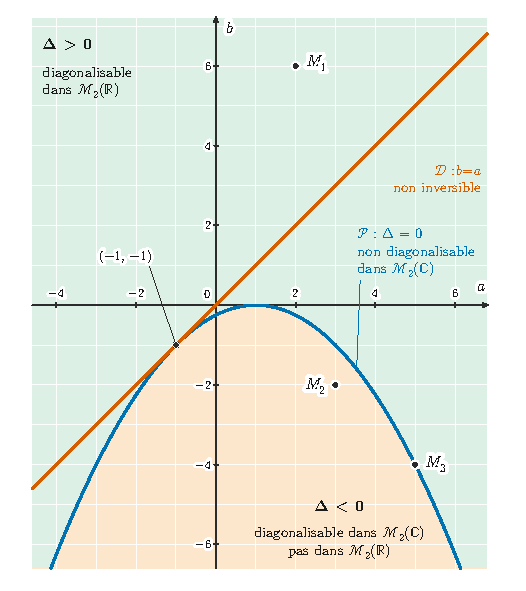
\includegraphics{figures/q8-plan-ab.pdf}
\caption*{Figure 1 --- plan (a, b) : la parabole 𝒫 (Δ = 0) sépare la région «
diagonalisable dans ℳ₂(ℝ) » de la région « diagonalisable dans ℳ₂(ℂ)
seulement » ; la droite 𝒟 des matrices non inversibles lui est tangente
en (−1, −1)}
\end{figure}

Sur la feuille millimétrée, on trace les axes avec leur origine et leurs graduations, en unité 1 cm, avec \(a\in[-5,7]\) et \(b\in[-8,8]\). On hachure les deux régions de deux façons différentes et l'on écrit la légende sur la feuille même.

\hypertarget{partie-b-un-couple-de-variables-aluxe9atoires}{%
\section{Partie B : Un couple de variables aléatoires}\label{partie-b-un-couple-de-variables-aluxe9atoires}}

On note \(c_{i,j}=P(X=x_i,Y=x_j)\), avec \((x_1,x_2,x_3)=(-1,0,1)\).

\hypertarget{a-2}{%
\subsection{1. (a)}\label{a-2}}

Pour tout \(i\), le coefficient d'indice \(i\) de \(CU\) est

\equationajustee{\begin{aligned}
(CU)_i&=\sum_{j=1}^3c_{i,j}\\
&=\sum_{j=1}^3P(X=x_i,Y=x_j).
\end{aligned}}

Comme \(Y(\Omega)=\{x_1,x_2,x_3\}\), les événements \((Y=x_1)\), \((Y=x_2)\), \((Y=x_3)\) forment un système complet d'événements. Par la formule des probabilités totales appliquée à ce système, cette somme vaut \(P(X=x_i)\).

Le vecteur \(CU\) est donc la colonne des \(P(X=x_i)\), et \(CU=\frac{1}{12}(4,5,3)^\top\).

\equationajustee{\boxed{\begin{aligned}
P(X=-1)&=\tfrac13\\
P(X=0)&=\tfrac5{12}\\
P(X=1)&=\tfrac14
\end{aligned}}}

\hypertarget{b-2}{%
\subsection{1. (b)}\label{b-2}}

Par définition de l'espérance d'une variable finie, et d'après (a),

\equationajustee{\begin{aligned}
V^\top CU&=\sum_{i=1}^3x_iP(X=x_i)\\
&=E(X).
\end{aligned}}

\equationajustee{\boxed{E(X)=-\tfrac13+\tfrac14=-\tfrac1{12}}}

\hypertarget{section-6}{%
\subsection{2.}\label{section-6}}

La loi de \(Y\) est donnée par le produit \(U^\top C\) (ligne des \(P(Y=x_j)\)), ou de façon équivalente par \(C^\top U\). L'espérance est donnée par \(E(Y)=U^\top CV\).

\equationajustee{U^\top C=\tfrac1{12}(4,4,4)=\big(\tfrac13,\tfrac13,\tfrac13\big).}

\equationajustee{\boxed{\begin{aligned}
P(Y=-1)&=\tfrac13\\
P(Y=0)&=\tfrac13\\
P(Y=1)&=\tfrac13
\end{aligned}}}

\textbf{\(Y\) suit la loi uniforme sur \(\{-1,0,1\}\).} Enfin, \(CV=\frac1{12}(1,-1,0)^\top\) et \(U^\top CV=0\).

\equationajustee{\boxed{E(Y)=U^\top CV=0}}

\hypertarget{section-7}{%
\subsection{3.}\label{section-7}}

On développe le produit :

\equationajustee{\begin{aligned}
V^\top CV&=\sum_{i=1}^3\sum_{j=1}^3x_i\,c_{i,j}\,x_j\\
&=\sum_{i=1}^3\sum_{j=1}^3x_ix_j\,P(X=x_i,Y=x_j).
\end{aligned}}

Par la formule de transfert appliquée au couple \((X,Y)\) et à la fonction \((u,v)\mapsto uv\), cette somme est \textbf{\(E(XY)\)}. Avec \(CV=\frac1{12}(1,-1,0)^\top\), on obtient :

\equationajustee{\boxed{V^\top CV=E(XY)=-\tfrac1{12}}}

\hypertarget{section-8}{%
\subsection{4.}\label{section-8}}

\equationajustee{\begin{aligned}
\mathrm{Cov}(X,Y)&=E(XY)-E(X)E(Y)\\
&=-\tfrac1{12}-\big(-\tfrac1{12}\big)\times0.
\end{aligned}}

\equationajustee{\boxed{\mathrm{Cov}(X,Y)=-\tfrac1{12}}}

\hypertarget{section-9}{%
\subsection{5.}\label{section-9}}

\textbf{\(X\) et \(Y\) ne sont pas indépendantes.} Deux justifications :

\begin{enumerate}
\def\labelenumi{\arabic{enumi}.}
\tightlist
\item
  Si \(X\) et \(Y\) étaient indépendantes, on aurait \(\mathrm{Cov}(X,Y)=0\), ce qui contredit la question 4.
\item
  \(P(X=-1,Y=-1)=c_{1,1}=\frac1{12}\), alors que \(P(X=-1)P(Y=-1)=\frac19\).
\end{enumerate}

On peut aussi remarquer que l'indépendance donnerait \(C=(CU)(U^\top C)\), matrice de rang \(1\). Or les colonnes \((1,2,1)^\top\) et \((2,1,1)^\top\) de \(12C\) ne sont pas colinéaires.

\hypertarget{section-10}{%
\subsection{6.}\label{section-10}}

Les événements \((X=x_i,Y=x_i)\), pour \(i\in\{1,2,3\}\), sont deux à deux incompatibles. Leur réunion est \((X=Y)\), puisque \(X\) et \(Y\) prennent leurs valeurs dans \(\{x_1,x_2,x_3\}\). Par additivité,

\equationajustee{\begin{aligned}
\mathrm{tr}(C)&=\sum_{i=1}^3c_{i,i}\\
&=P(X=Y).
\end{aligned}}

Numériquement, \(c_{1,1}+c_{2,2}+c_{3,3}=\frac{1+2+1}{12}\).

\equationajustee{\boxed{\begin{aligned}
\mathrm{tr}(C)&=P(X=Y)\\
&=\tfrac13
\end{aligned}}}

\hypertarget{partie-c-des-variables-aluxe9atoires-dans-une-matrice}{%
\section{Partie C : Des variables aléatoires dans une matrice}\label{partie-c-des-variables-aluxe9atoires-dans-une-matrice}}

\hypertarget{a-3}{%
\subsection{1. (a)}\label{a-3}}

D'après A.5, \(M(A,B)\) est inversible si et seulement si \(A\neq B\). Les événements \(\big(M(A,B)\text{ inversible}\big)\) et \((A\neq B)\) sont donc égaux. Avec \(A=X\), \(B=Y\) et B.6 :

\equationajustee{\begin{aligned}
P\big(M(A,B)\text{ inversible}\big)&=1-P(X=Y)\\
&=1-\tfrac13.
\end{aligned}}

\equationajustee{\boxed{P\big(M(A,B)\text{ inversible}\big)=\tfrac23}}

\hypertarget{b-3}{%
\subsection{1. (b)}\label{b-3}}

D'après A.7, \(M(A,B)\) n'est diagonalisable ni dans \({\mathcal{M}}_2(\mathbb{R})\) ni dans \({\mathcal{M}}_2(\mathbb{C})\) si et seulement si \(\Delta(A,B)=0\), avec \(\Delta(A,B)=(A-1)^2+4B\). Sur \(\{-1,0,1\}^2\) :

\begin{itemize}
\tightlist
\item
  pour \(a=-1\), \(4+4b=0\) donne \(b=-1\) ;
\item
  pour \(a=0\), \(1+4b=0\) n'a pas de solution dans \(\{-1,0,1\}\) ;
\item
  pour \(a=1\), \(4b=0\) donne \(b=0\).
\end{itemize}

Les deux événements \((X=-1,Y=-1)\) et \((X=1,Y=0)\) sont incompatibles, donc

\equationajustee{\begin{aligned}
P\big(\Delta(A,B)=0\big)&=c_{1,1}+c_{3,2}\\
&=\tfrac1{12}+\tfrac1{12}.
\end{aligned}}

\equationajustee{\boxed{P\big(\Delta(A,B)=0\big)=\tfrac16}}

\hypertarget{section-11}{%
\subsection{2.}\label{section-11}}

Comme \(A\) et \(B\) sont à valeurs dans \(H\), on a l'égalité d'événements \((A=B)=\bigcup_{k\in H}\big((A=k)\cap(B=k)\big)\).

En effet, si \(A(\omega)=B(\omega)\), cette valeur commune est un élément \(k\) de \(H\), et la réciproque est immédiate.

Ces événements sont deux à deux incompatibles, car \((A=k)\cap(A=k')=\varnothing\) pour \(k\neq k'\). Ils sont en nombre au plus dénombrable, car \(H\subset\mathbb{N}\).

Par \(\sigma\)-additivité, puis par indépendance de \(A\) et \(B\) :

\equationajustee{\begin{aligned}
P(A=B)&=\sum_{k\in H}P\big((A=k)\cap(B=k)\big)\\
&=\boxed{\sum_{k\in H}P(A=k)P(B=k)}.
\end{aligned}}

\hypertarget{a-4}{%
\subsection{3. (a)}\label{a-4}}

On note \(q=1-p\).

\equationajustee{\boxed{\begin{aligned}{}&A(\Omega)=[\![0;n]\!],\\
&\forall k\in[\![0;n]\!],\ P(A=k)=\binom nk p^kq^{n-k}
\end{aligned}}}

\hypertarget{b-4}{%
\subsection{3. (b)}\label{b-4}}

\equationajustee{\boxed{\begin{aligned}{}&B(\Omega)={\mathbb{N}}^*,\\
&\forall k\in{\mathbb{N}}^*,\ P(B=k)=r(1-r)^{k-1}
\end{aligned}}}

\hypertarget{c}{%
\subsection{3. (c)}\label{c}}

\(M(A,B)\) est non inversible si et seulement si \(A=B\) (A.5). Les variables \(A\) et \(B\) sont indépendantes et toutes deux à valeurs dans \(H=\mathbb{N}\), donc la question 2 s'applique.

On a \(P(B=0)=0\), et \(P(A=k)=0\) pour \(k>n\). Il reste les indices \(k\in[\![1;n]\!]\) :

\equationajustee{\begin{aligned}
P(A=B)&=\sum_{k=1}^n\binom nk p^k(1-p)^{n-k}\,r(1-r)^{k-1}\\
&=\frac{r}{1-r}\sum_{k=1}^n\binom nk\big(p(1-r)\big)^k(1-p)^{n-k}.
\end{aligned}}

On complète la somme avec le terme \(k=0\), qui vaut \((1-p)^n\), et on le retranche. La formule du binôme de Newton, avec \(p(1-r)+(1-p)=1-pr\), donne

\equationajustee{\begin{aligned}
\sum_{k=1}^n\binom nk\big(p(1-r)\big)^k(1-p)^{n-k}&=\big(p(1-r)+1-p\big)^n-(1-p)^n\\
&=(1-pr)^n-(1-p)^n.
\end{aligned}}

\equationajustee{\boxed{P\big(M(A,B)\text{ non inversible}\big)=\frac{r}{1-r}\Big[(1-pr)^n-(1-p)^n\Big]}}

\hypertarget{a-5}{%
\subsection{4. (a)}\label{a-5}}

\equationajustee{\boxed{\begin{aligned}{}&A(\Omega)=\mathbb{N},\\
&\forall k\in\mathbb{N},\ P(A=k)=e^{-\lambda}\frac{\lambda^k}{k!}
\end{aligned}}}

\hypertarget{b-5}{%
\subsection{4. (b)}\label{b-5}}

Si \(Z\sim\mathcal{P}(\theta)\), alors pour tout \(t\in\mathbb{R}\),

\equationajustee{\begin{aligned}
G_Z(t)&=\sum_{k\ge0}e^{-\theta}\frac{(\theta t)^k}{k!}\\
&=e^{\theta(t-1)}.
\end{aligned}}

Les variables \(A\) et \(C=-B\) sont à valeurs dans \(\mathbb{N}\).

Elles sont indépendantes, puisque \(C\) est une fonction de \(B\) et que \(A\) et \(B\) sont indépendantes. La fonction génératrice d'une somme de variables indépendantes est le produit des fonctions génératrices :

\equationajustee{\begin{aligned}
G_{A+C}(t)&=G_A(t)\,G_C(t)\\
&=e^{\lambda(t-1)}e^{\mu(t-1)}\\
&=e^{(\lambda+\mu)(t-1)}.
\end{aligned}}

La fonction génératrice caractérise la loi d'une variable à valeurs dans \(\mathbb{N}\), d'où

\equationajustee{\boxed{A+C\sim\mathcal{P}(\lambda+\mu)}}

\hypertarget{c-1}{%
\subsection{4. (c)}\label{c-1}}

D'après A.5, \(M(A,B)\) est inversible si et seulement si \(A\neq B\), c'est-à-dire \(A+C\neq0\). D'après (b),

\equationajustee{\begin{aligned}
P\big(M(A,B)\text{ inversible}\big)&=1-P(A+C=0)\\
&=1-e^{-(\lambda+\mu)}.
\end{aligned}}

\equationajustee{\boxed{P\big(M(A,B)\text{ inversible}\big)=1-e^{-(\lambda+\mu)}}}

\hypertarget{section-12}{%
\subsection{5.}\label{section-12}}

\(M(A,B)\) est non inversible si et seulement si \(A=B\) (A.5). Les variables \(A\) et \(B\) sont indépendantes et à valeurs dans \(\mathbb{N}\) : on applique la question 2 avec \(H=\mathbb{N}\).

\equationajustee{\begin{aligned}
P(A=B)&=\sum_{k=0}^{+\infty}e^{-\lambda}\frac{\lambda^k}{k!}\,e^{-\mu}\frac{\mu^k}{k!}\\
&=\sum_{k=0}^{+\infty}\frac{(\lambda\mu)^k}{(k!)^2}e^{-(\lambda+\mu)}.
\end{aligned}}

\equationajustee{\boxed{P\big(M(A,B)\text{ non inversible}\big)=I}}

La série converge, puisque ses termes sont positifs et majorés par ceux de la série exponentielle de \(\lambda\mu\).

\hypertarget{a-6}{%
\subsection{6. (a)}\label{a-6}}

Tous les termes de \(R_n\) sont positifs, donc \(R_n\geqslant0\) et \(|R_n|=R_n\).

Pour \(k\geqslant n+1\), on a \(k!\geqslant(n+1)!\), donc \((k!)^2\geqslant(n+1)!\,k!\). Il vient

\equationajustee{\begin{aligned}
|R_n|&\leqslant\frac{e^{-(\lambda+\mu)}}{(n+1)!}\sum_{k=n+1}^{+\infty}\frac{(\lambda\mu)^k}{k!}\\
&\leqslant\frac{e^{-(\lambda+\mu)}}{(n+1)!}\sum_{k=0}^{+\infty}\frac{(\lambda\mu)^k}{k!}\\
&=\frac{e^{\lambda\mu-(\lambda+\mu)}}{(n+1)!}.
\end{aligned}}

La deuxième inégalité vient de ce que l'on ajoute les termes positifs d'indices \(0\) à \(n\).

\equationajustee{\boxed{\forall n\geqslant0,\quad |R_n|\leqslant\frac{1}{(n+1)!}e^{\lambda\mu-(\lambda+\mu)}}}

\hypertarget{b-6}{%
\subsection{6. (b)}\label{b-6}}

Notons \(S_n\) la somme partielle d'indice \(n\) de \(I\), de sorte que \(I-S_n=R_n\).

Dès que le majorant de 6(a) est inférieur ou égal à \texttt{eps}, \(S_n\) est une valeur approchée de \(I\) à \texttt{eps} près. Ce majorant tend vers \(0\) quand \(n\) tend vers l'infini, donc la boucle termine.

\begin{lstlisting}[language=Python]
from math import exp, factorial

def val_app(eps):
    # n : indice du dernier terme ajouté ; S : somme partielle S_n
    n = 0
    S = exp(-(la + mu))                                   # S_0 : terme k = 0
    # tant que le majorant de |R_n| (question 6.a) dépasse eps, on ajoute un terme
    while exp(la * mu - (la + mu)) / factorial(n + 1) > eps:
        n = n + 1
        S = S + (la * mu) ** n / factorial(n) ** 2 * exp(-(la + mu))   # S devient S_n
    return S                                              # |I - S_n| <= eps
\end{lstlisting}

Pour \(\lambda=1\), \(\mu=2\) et \texttt{eps\ =\ 1e-5}, la boucle s'arrête à \(n=7\) et la fonction renvoie \(0{,}211712\ldots\)

\hypertarget{c-2}{%
\subsection{6. (c)}\label{c-2}}

Les variables globales \texttt{la} et \texttt{mu} étant affectées, on ajoute l'instruction :

\begin{lstlisting}[language=Python]
print(val_app(10**-5))
\end{lstlisting}

\hypertarget{a-7}{%
\subsection{7. (a)}\label{a-7}}

\(J_i\) prend les valeurs \(0\) et \(1\) : c'est une variable de Bernoulli. Son paramètre est

\equationajustee{\begin{aligned}
P(J_i=1)&=P\big(M(A,B)\text{ non inversible}\big)\\
&=I,
\end{aligned}}

d'après la question 5.

\equationajustee{\boxed{J_i\sim\mathcal{B}(I)\quad\text{(loi de Bernoulli de \text{paramètre} } I)}}

\hypertarget{b-7}{%
\subsection{7. (b)}\label{b-7}}

La somme définissant \(K_N\) porte sur les \(J_k\) (l'indice \(J_i\) de l'énoncé est une coquille sans incidence).

Les simulations sont indépendantes, donc \(J_1,\dots,J_N\) sont des variables indépendantes, toutes de loi \(\mathcal{B}(I)\).

D'après le cours, si \(J_1,\dots,J_N\) sont indépendantes de loi de Bernoulli de paramètre \(I\), alors \(J_1+\dots+J_N\) suit la loi binomiale de paramètres \(N\) et \(I\).

\equationajustee{\boxed{K_N\sim\mathcal{B}(N,I)}}

\hypertarget{c-3}{%
\subsection{7. (c)}\label{c-3}}

On a \(E(K_N)=NI\) et \(V(K_N)=NI(1-I)\). Par linéarité de l'espérance et par la relation \(V(aZ)=a^2V(Z)\) :

\equationajustee{\boxed{\begin{aligned}
E(\overline{K_N})&=I\\
V(\overline{K_N})&=\frac{I(1-I)}{N}
\end{aligned}}}

\hypertarget{d}{%
\subsection{7. (d)}\label{d}}

\(\overline{K_N}\) est une variable finie, donc elle admet une variance. L'inégalité de Bienaymé-Tchebychev donne, pour tout \(\varepsilon>0\),

\equationajustee{P\big(|\overline{K_N}-I|\geqslant\varepsilon\big)\leqslant\frac{I(1-I)}{N\varepsilon^2}.}

Par ailleurs, la forme canonique donne la majoration

\equationajustee{I(1-I)=\frac14-\Big(I-\frac12\Big)^2\leqslant\frac14.}

\equationajustee{\boxed{\forall\varepsilon>0,\quad P\big(|\overline{K_N}-I|\geqslant\varepsilon\big)\leqslant\frac1{4N\varepsilon^2}}}

\hypertarget{e}{%
\subsection{7. (e)}\label{e}}

L'événement \(\big(I\in[\overline{K_N}-\varepsilon\,;\,\overline{K_N}+\varepsilon]\big)\) est l'événement \(\big(|\overline{K_N}-I|\leqslant\varepsilon\big)\).

Il contient l'événement contraire de \(\big(|\overline{K_N}-I|\geqslant\varepsilon\big)\), qui est \(\big(|\overline{K_N}-I|<\varepsilon\big)\). Par croissance de \(P\), puis par 7(d) :

\equationajustee{\begin{aligned}
P\big(I\in[\overline{K_N}-\varepsilon\,;\,\overline{K_N}+\varepsilon]\big)&\geqslant1-P\big(|\overline{K_N}-I|\geqslant\varepsilon\big)\\
&\geqslant1-\frac1{4N\varepsilon^2}.
\end{aligned}}

\equationajustee{\boxed{\forall\varepsilon>0,\quad P\big(I\in[\overline{K_N}-\varepsilon\,;\,\overline{K_N}+\varepsilon]\big)\geqslant1-\frac1{4N\varepsilon^2}}}

\hypertarget{f}{%
\subsection{7. (f)}\label{f}}

On a \(N=10^5\) et la réalisation observée de \(\overline{K_N}\) vaut

\equationajustee{\overline{K_N}=\frac{21\,357}{100\,000}=0{,}21357.}

\begin{itemize}
\item
  Pour \(\varepsilon=10^{-2}\) : \(\frac{1}{4N\varepsilon^2}=\frac{1}{40}=0{,}025\).

  \textbf{Avec une probabilité au moins égale à \(0{,}975\), l'intervalle aléatoire \([\overline{K_N}-0{,}01\,;\,\overline{K_N}+0{,}01]\) contient \(I\).}

  Pour cette simulation, il vaut \([0{,}20357\,;\,0{,}22357]\) : c'est un intervalle de confiance de \(I\) au niveau \(97{,}5\,\%\). Arrondi vers l'extérieur, il devient \([0{,}203\,;\,0{,}224]\).
\item
  Pour \(\varepsilon=10^{-3}\) : \(\frac{1}{4N\varepsilon^2}=2{,}5\), et le minorant \(1-2{,}5=-1{,}5\) est négatif. Une probabilité est toujours positive : \textbf{l'inégalité ne donne aucune information.}
\end{itemize}

À titre de contrôle, la valeur calculée en 6(b) est \(I\approx0{,}21171\) ; elle appartient bien au premier intervalle.

\hypertarget{partie-d-un-deuxiuxe8me-couple-de-variables-aluxe9atoires}{%
\section{Partie D : Un deuxième couple de variables aléatoires}\label{partie-d-un-deuxiuxe8me-couple-de-variables-aluxe9atoires}}

On note \(\alpha=\big(P(X=x_i)\big)_{1\le i\le n}\) et \(\beta=\big(P(Y=y_j)\big)_{1\le j\le n}\), vus comme vecteurs colonnes.

En généralisant la partie B, on a \(QU=\alpha\) et \(Q^\top U=\beta\), et les coordonnées de \(\alpha\) et de \(\beta\) sont de somme \(1\).

\hypertarget{a-8}{%
\subsection{1. (a)}\label{a-8}}

Par indépendance, \(q_{i,j}=\alpha_i\beta_j\) pour tous \(i,j\), donc \(Q=\alpha\beta^\top\).

Toutes les colonnes de \(Q\) sont colinéaires à \(\alpha\), donc \(\mathrm{rg}\,Q\leqslant1\).

De plus, \(\alpha\neq0\) et \(\beta\neq0\), puisque leurs coordonnées sont de somme \(1\). Donc \(Q\neq0\) et \(\mathrm{rg}\,Q\geqslant1\).

\equationajustee{\boxed{\mathrm{rg}\,Q=1}}

\hypertarget{b-8}{%
\subsection{1. (b)}\label{b-8}}

Le cas \(n=1\) est à part : \(Q=(1)\), et la seule valeur propre est \(1\). On suppose désormais \(n\geqslant2\).

\begin{itemize}
\item
  Par le théorème du rang, \(\dim\ker Q=n-1\geqslant1\). Donc \textbf{\(0\) est valeur propre de \(Q\), avec un sous-espace propre de dimension \(n-1\)}. La dimension d'un sous-espace propre est majorée par la multiplicité de la valeur propre, donc cette multiplicité est au moins \(n-1\).
\item
  On a \(\beta^\top\alpha=\sum_i\alpha_i\beta_i=\sum_iq_{i,i}=\mathrm{tr}\,Q\). Il vient \(Q^2=\alpha(\beta^\top\alpha)\beta^\top=\mathrm{tr}(Q)\,Q\).
\item
  Si \(Qx=\lambda x\) avec \(x\neq0\), on calcule \(Q^2x\) de deux façons (\(Q^2=\mathrm{tr}(Q)\,Q\)) :

  \equationajustee{\lambda^2x=\mathrm{tr}(Q)\,\lambda x.}

  Comme \(x\neq0\), il vient \(\lambda\big(\lambda-\mathrm{tr}(Q)\big)=0\) : \textbf{les seules valeurs propres possibles sont \(0\) et \(\mathrm{tr}\,Q\)}.
\item
  \(Q\) est trigonalisable dans \({\mathcal{M}}_n(\mathbb{C})\), donc sa trace est la somme de ses valeurs propres complexes comptées avec multiplicité ; cette somme vaut \(\mathrm{tr}\,Q\), d'où \(\chi_Q=X^{n-1}\big(X-\mathrm{tr}\,Q\big)\).
\end{itemize}

\equationajustee{\boxed{\begin{aligned}{}&\text{si } \mathrm{tr}\,Q\neq0 :\ 0 \text{ de \text{multiplicité} } n-1 \text{ et } \mathrm{tr}\,Q \text{ de \text{multiplicité} } 1\ ;\\
&\text{si } \mathrm{tr}\,Q=0 :\ 0 \text{ seule, de \text{multiplicité} } n
\end{aligned}}}

\hypertarget{c-4}{%
\subsection{1. (c)}\label{c-4}}

Ici \(\mathrm{tr}\,Q=\sum_i\alpha_i\beta_i\), avec \(\alpha_i>0\) pour tout \(i\), et les \(\beta_i\) positifs de somme \(1\).

Il existe donc \(i_0\) tel que \(\beta_{i_0}>0\), ce qui donne \(\mathrm{tr}\,Q\geqslant\alpha_{i_0}\beta_{i_0}>0\).

Or \(Q\alpha=\alpha(\beta^\top\alpha)=(\mathrm{tr}\,Q)\,\alpha\) avec \(\alpha\neq0\). Donc \(\mathrm{tr}\,Q\) est valeur propre, et son sous-espace propre est de dimension au moins \(1\).

La somme des dimensions des sous-espaces propres vaut alors au moins \((n-1)+1=n\), d'où

\equationajustee{\boxed{Q \text{ est diagonalisable, semblable \text{à} } \mathrm{diag}(\mathrm{tr}\,Q,0,\dots,0)}}

Pour \(n=1\), \(Q=(1)\) est diagonale.

\hypertarget{d-1}{%
\subsection{1. (d)}\label{d-1}}

Prenons \(x_i=y_i=i\) pour \(i\in[\![1;4]\!]\) et \(\Omega=[\![1;4]\!]^2\), muni de la probabilité \(P(\{(i,j)\})=a_ib_j\), avec

\equationajustee{\begin{aligned}
a&=\big(\tfrac12,\tfrac12,0,0\big),\\
b&=\big(0,0,\tfrac12,\tfrac12\big).
\end{aligned}}

Posons \(X(i,j)=x_i\) et \(Y(i,j)=y_j\). On a bien \(X(\Omega)=Y(\Omega)=\{1,2,3,4\}\).

Les variables \(X\) et \(Y\) sont indépendantes, avec \(P(X=x_i)=a_i\) et \(P(Y=y_j)=b_j\).

\(X\) suit la loi uniforme sur \(\{1,2\}\) et \(Y\) la loi uniforme sur \(\{3,4\}\), donc aucune n'est constante. On a cependant \(P(X=3)=P(X=4)=0\).

\equationajustee{Q=\frac14\begin{pmatrix}0&0&1&1\\0&0&1&1\\0&0&0&0\\0&0&0&0\end{pmatrix}.}

Ses coefficients sont positifs, de somme \(1\) : c'est bien la matrice d'une loi conjointe, et elle est de rang \(1\).

On a \(\mathrm{tr}\,Q=0\), donc \(Q^2=\mathrm{tr}(Q)\,Q=0\) et \(0\) est la seule valeur propre. Si \(Q\) était diagonalisable, elle serait semblable à la matrice nulle, donc nulle. Comme \(Q\neq0\), \textbf{\(Q\) n'est pas diagonalisable.}

Cet exemple est nécessairement de ce type. Pour \(X\) et \(Y\) indépendantes, la non-diagonalisabilité impose \(\mathrm{tr}\,Q=0\), donc certaines valeurs \(x_i\) doivent être prises avec une probabilité nulle.

\hypertarget{section-13}{%
\subsection{2.}\label{section-13}}

Supposons \(\mathrm{rg}\,Q=1\). L'image de \(Q\) est une droite \(\mathrm{Vect}(u)\).

Chaque colonne \(Qe_j\) s'écrit \(v_ju\). On a donc \(Q=uv^\top\), avec \(u,v\in{\mathbb{R}}^n\).

On pose \(s=\sum_jv_j\) et \(t=\sum_iu_i\). En généralisant B.1 et B.2 :

\equationajustee{\begin{aligned}
\alpha&=QU=u\,(v^\top U)=s\,u,\\
\beta&=Q^\top U=v\,(u^\top U)=t\,v.
\end{aligned}}

La somme de toutes les probabilités jointes vaut \(1\), donc

\equationajustee{\begin{aligned}
1&=U^\top QU\\
&=(U^\top u)(v^\top U)\\
&=ts.
\end{aligned}}

Par suite,

\equationajustee{\begin{aligned}
\alpha\beta^\top&=st\,uv^\top\\
&=Q.
\end{aligned}}

Autrement dit, pour tous \((i,j)\), \(P(X=x_i,Y=y_j)=P(X=x_i)\,P(Y=y_j)\).

\equationajustee{\boxed{\mathrm{rg}\,Q=1\implies X \text{ et } Y \text{ \text{indépendantes}}}}

Avec 1(a), on obtient l'équivalence : \textbf{\(X\) et \(Y\) sont indépendantes si et seulement si \(\mathrm{rg}\,Q=1\).}

\end{document}
